\begin{question}
  \hspace*{\fill} [Note Maximale: 2]\par
  \medskip
  \noindent Soit $f(x) = Sin(ex)$ pour $0 \le x \le 1,5$ .\par
  \medskip
  \begin{center} % or flushleft or flushright
    \noindent Le diagramme suivant montre la représentation graphique de $f$.\par
    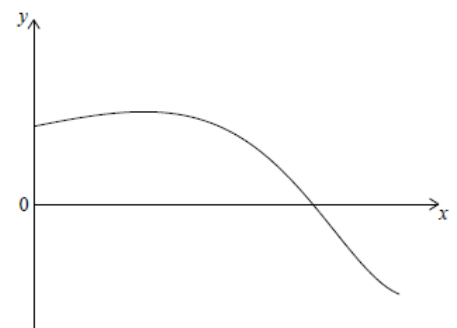
\includegraphics[scale=0.4]{diagramme_x19}\par
  \end{center} % or flushleft or flushright

  \medskip
  \noindent Trouvez l'abscisse à l'origine de la représentation graphique de $f$.\hspace*{\fill} [2]\par
  
\end{question}
